\documentclass{article} % For LaTeX2e
\usepackage{nips15submit_e,times}
\usepackage{hyperref}
\usepackage{url}
\usepackage{graphicx}
%\documentstyle[nips14submit_09,times,art10]{article} % For LaTeX 2.09


\title{Neural Embedding for Market Basket Analysis}

\author{ Bill Chambers \thanks{This work is part of Computer Science 289 Course} \\
School of Information \\
University of California Berkeley\\
Berkeley, CA 94720 \\
\texttt{wachambers@berkeley.edu} \\
\AND
Yu "Andy" Wang \\
Department of Computer Science \\
University of California Berkeley\\
Berkeley, CA 94720 \\
\texttt{andyatcal@berkeley.edu}
}

% The \author macro works with any number of authors. There are two commands
% used to separate the names and addresses of multiple authors: \And and \AND.
%
% Using \And between authors leaves it to \LaTeX{} to determine where to break
% the lines. Using \AND forces a linebreak at that point. So, if \LaTeX{}
% puts 3 of 4 authors names on the first line, and the last on the second
% line, try using \AND instead of \And before the third author name.

\newcommand{\fix}{\marginpar{FIX}}
\newcommand{\new}{\marginpar{NEW}}

\nipsfinalcopy % Uncomment for camera-ready version

\begin{document}

\maketitle


\begin{abstract}

\end{abstract}

\section{Introduction}

Our research stemmed from a lecture by Professor Efros in which a student asked,  Professor, if we re given a matrix with lots of categorical variables, what s the best way to approach this style of problem with a neural network?  His response was that our focus should be a Random Forest or a tree-based method. 

Our group took this as a challenge and decided to pursue this open research question. We recognize that a tree-based method is not only the obvious choice, but would set a strong baseline for us to beat. We decided to pursue this research area by finding a competition featuring this kind of dataset.

\subsection{Challenge and Data}

The challenge that we competed in was a challenge put on Walmart on the Kaggle competition website[https://www.kaggle.com/c/walmart-recruiting-trip-type-classification]. Walmart created a dataset of transactions during  visits by individual customers. They then classified these into a variety of different "Trip Types" according to their perception of the motivation of the customer visits in order to improve the segmentation process and improve customer experience.

As mentioned, the raw data is transactional in nature - being a collection of purchased items making it a customer transaction is a collection of purchased items and corresponds to one unique “trip type”. Every purchased item (or every row in the dataset) have 6 features, including 5 categorical features and 1 numerical feature. One example of customer visit (of VisitNumber = 10) in shown in the table below.

\begin{center}
  \begin{tabular}{ c | c | c | c | c | c | c}
    TripType & VisitNumber & Weekday & Upc & Scans & Department & FinelineNumber \\
 8 & 10 & Friday & 6414410235 & 1 & DSD Grocery & 2008 \\
 8 & 10 & Friday & 2800053970 & 1 & Candy, Tobacco... & 115 \\
 8 & 10 & Friday & 7794800902 & 1 & DSD Grocery & 7950 \\
  \end{tabular}
\end{center}

TripType is the label or our classification target. The other features provided are: (a) Weekday, the weekday of the trip; (b) ScanCount, the number of items purchased [if positive] or the number of items purchased then returned [if negative]; (c) three levels of granularity for item categorization: DepartmentDescription, FinelineNumber, and Upc. 

There exist 68 unique department descriptions. They define the highest level category, the department from which the item was purchased. The middle category is the "Fineline Number" a categorization scheme created by Walmart to provide a middle level of granularity. Fineline number is a four digit number that refers to a group of items within a department which show similar sales patterns. It is determined by sales patterns and that each product is placed accurately within a fineline to maximize sales. (http://blog.8thandwalton.com/2014/06/supplier-glossary-fineline/) There are approximately 5600 unique Fineline Numbers in the training set. 

UPC[Universal Product Code] is a barcode symbology for tracking purchased items. There are about 98000 uniques UPCs in the dataset, with each of them corresponds to a specific product. This is even more than our train sample size. It generally uses the common form of UPC-A and is of 12 numerical digits. “Every UPC-A barcode follows the pattern SLLLLLLMRRRRRRE.” S, M,and E stands for the start, middle, and end non-numerical guard bars. 

L (left) and R (right) sections represent the 12 numerical digits of UPC-A.(https://en.wikipedia.org/wiki/Universal\_Product\_Code/)

However, not all UPC in the dataset is in this form. The length of UPC varies from 3 to 12, indicating that Walmart is using UPC in its own standard or trimming the starting 0 in UPC-A standards.

The core challenge with regard to this dataset is the absence of numerical data. While scan count exhibits so numerical basis, it also represents returns, making it categorical. Creating a binary representation of the data creates extremely sparse matrices making modeling difficult and reinforcing our understanding of the curse of dimensionality.

\section{Previous Research for Handling Categorical Data}
\label{gen_inst}
References:
http://www-users.cs.umn.edu/~sboriah/PDFs/BoriahBCK2008.pdf
http://www.umass.edu/landeco/teaching/multivariate/readings/McCune.and.Grace.2002.chapter6.pdf
http://www.cc.gatech.edu/~fli/chebyshev\_cvpr12.pdf
http://papers.nips.cc/paper/5075-sign-cauchy-projections-and-chi-square-kernel.pdf
http://www.mtome.com/Publications/CiML/CiML-v3-book.pdf
http://www.marc-boulle.fr/publications/BoulleMLDM05.pdf (Marc Boullé)

https://www3.nd.edu/~dial/papers/ASONAMJ10.pdf

http://www.emeraldinsight.com/doi/abs/10.1108/eb026526



\section{Process and Benchmarks}
\label{headings}

Our process was attack this problem from two directions. Firstly we wanted to get baseline results from a variety of methods including Random Forests, Logistic Regression, K-Nearest Neighbors, Linear Support Vector Classifiers. We experimented with extremely limited transformations from the raw data in order to better understand out of the box results. This included leveraging only the Scan Count and Department Description columns. We tuned each of these methods using a grid search methodology leveraging k-fold cross validation (k=3) and comparing their results on a validation set. Our initial results were relatively consistent across the various methods based on the exact same training and validation sets.

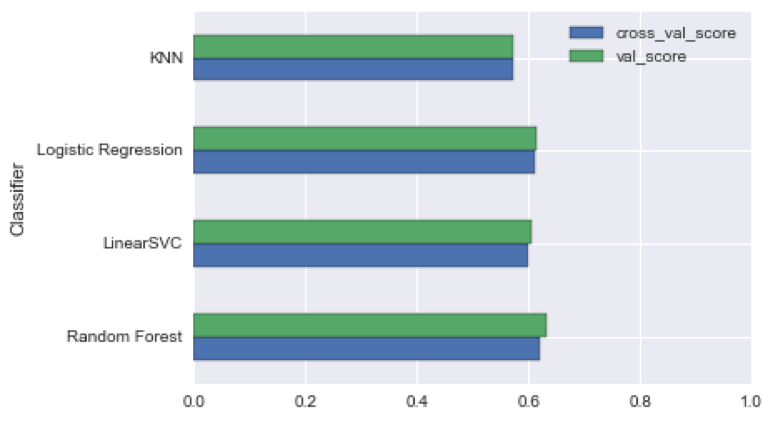
\includegraphics[scale=0.4]{comparison_baseline.png} 

These methods all yielded similar results on the Kaggle public test set. This stimulated interesting discussion within our group as we expected our Random Forest classifier to perform much better than the other methods, while it only yielded nominally improved results. We attribute this again to the sparseness of the data as well as the implementation that we had used.

It was at this point that we decided to focus completely on non-tree based methods and start working our original research objective, how to leverage feature transformations in order to compete with random forests.


\section{A Novel Approach: Neural Embeddings for Market Basket Analysis}

After exploring the literature, we identified an unexplored research area. While building networks between products is not uncommon, typically these networks are grown manually or through more direct probabilistic modeling. CITATION HERE=https://www3.nd.edu/~dial/papers/ASONAMJ10.pdf. However after experimentation, we identified an underlying structure in our market baskets. Rather than thinking about them as products, we borrowed from statistical natural language processing and thought of them as words or tokens. This leverages the concept of an latent network in the data, but also the concept of a semantic structure to the data. This inspired us to turn the baskets into bags of words that included the Fineline Number and the Department description.

After creating this structure, we learned a Word2Vec model (CITATION) using the continuous bag of words approach in order to attempt to extract the underlying product network and relationships. We then use this information when creating our model by adding the similar "words" into the current market basket. After which we borrow for NLP again and perform a TFIDF (http://www.emeraldinsight.com/doi/abs/10.1108/eb026526) feature weighting in order to reweight the features. We then pass this into a simple two layeer neural network tuned with cross entropy loss. Doing so allowed us to improve on our naive models in terms of both test and validation accuracy by several points.

We think that this approach holds much promise.


\section{Data Exploration and Categorization}
A better understanding of the dataset helps feature extraction and better pre-processing for training. In this dataset, we explore the meaning of the label, TripType, and why Walmart assigns certain trip types to some transactions. A quick dive into the dataset offers the following facts:
(1) All transactions with negative total scan count is assigned with TripType 999.
(2) Transactions with more than 50% of Financial services and number of scan count smaller than 4 are assigned with TripType 3.
(3) Transactions with more than 50% of Pharmacy are generally assigned to TripType 4 and 5, where 4 is of pharmacy OTC and 5 is of misture of pharmacy OTC, RC and Optical.
(4) Food and drinks transactions are assigned with TripType 6, 7, and 8, where 6 is on snacks and liquor, 7 is on main meals (either cooked or uncooked), and 8 is a mixture of stuffs in 6 or 7 but with a small amount.
(5) A small amount mixture of living products, e.g., home, auto, electronics, clothing, shoes, beauty is assigned with TripType 9.
(6) A medium level of scans of lawn garden, households goods, cook and dine and toys are assigned with TriyType 12.
…
A generalization from these facts is that TripType is basically determined by (a) the size of the transaction (i.e. the total number of scan counts), (b) the structure of the transaction (i.e. the proportion of scan count on each department), and (c) the impurity of the transaction (i.e. entropy). 
Figure X shows the distribution of trip types on its average transaction size and transaction impurity.

\section{Future Research}


\section{Conclusion}
In this paper we introduce the concept of a 


\subsubsection*{Acknowledgments}

Use unnumbered third level headings for the acknowledgments. All
acknowledgments go at the end of the paper. Do not include 
acknowledgments in the anonymized submission, only in the 
final paper. 

\subsubsection*{References}

\bibliography{references.bib}
\bibliographystyle{small}

FIX ME 
References follow the acknowledgments. Use unnumbered third level heading for
the references. Any choice of citation style is acceptable as long as you are
consistent. It is permissible to reduce the font size to `small' (9-point) 
when listing the references. {\bf Remember that this year you can use
a ninth page as long as it contains \emph{only} cited references.}

\small{
[1] Alexander, J.A. \& Mozer, M.C. (1995) Template-based algorithms
for connectionist rule extraction. In G. Tesauro, D. S. Touretzky
and T.K. Leen (eds.), {\it Advances in Neural Information Processing
Systems 7}, pp. 609-616. Cambridge, MA: MIT Press.

[2] Bower, J.M. \& Beeman, D. (1995) {\it The Book of GENESIS: Exploring
Realistic Neural Models with the GEneral NEural SImulation System.}
New York: TELOS/Springer-Verlag.



\end{document}